\documentclass{beamer}
\usetheme{Boadilla}

\makeatother
\setbeamertemplate{footline}
{
    \leavevmode%
    \hbox{%
    \begin{beamercolorbox}[wd=.4\paperwidth,ht=2.25ex,dp=1ex,center]{author in head/foot}%
        \usebeamerfont{author in head/foot}\insertshortauthor
    \end{beamercolorbox}%
    \begin{beamercolorbox}[wd=.55\paperwidth,ht=2.25ex,dp=1ex,center]{title in head/foot}%
        \usebeamerfont{title in head/foot}\insertshorttitle
    \end{beamercolorbox}%
    \begin{beamercolorbox}[wd=.05\paperwidth,ht=2.25ex,dp=1ex,center]{date in head/foot}%
        \insertframenumber{}
    \end{beamercolorbox}}%
    \vskip0pt%
}
\makeatletter
\setbeamertemplate{navigation symbols}{}

\usepackage[T1]{fontenc}
\usepackage{lmodern}
\usepackage{amssymb,amsmath}
\renewcommand{\familydefault}{\sfdefault}

\usepackage{mathtools}
\usepackage{graphicx}
\usepackage{threeparttable}
\usepackage{booktabs}
\usepackage{siunitx}
\sisetup{parse-numbers=false}

%\setlength{\OuterFrameSep}{-2pt}
%\makeatletter
%\preto{\@verbatim}{\topsep=-10pt \partopsep=-10pt }
%\makeatother

\title[Lecture 5:\ Logit Model II]{Lecture 5:\ Logit Model II}
\author[ResEcon 703:\ Advanced Econometrics]{ResEcon 703:\ Topics in Advanced Econometrics}
\date{Matt Woerman\\University of Massachusetts Amherst}

\begin{document}

{\setbeamertemplate{footline}{} 
\begin{frame}[noframenumbering]
    \titlepage
\end{frame}
}

\begin{frame}\frametitle{Agenda}
    Last time
    \begin{itemize}
        \item Logit Model
    \end{itemize}
    \vspace{2ex}
    Today
    \begin{itemize}
    	\item More Logit Properties
    	\item Multinomial Logit Model Example in R
    	\item Adamowicz et al. (1994)
    \end{itemize}
    \vspace{2ex}
    Upcoming
    \begin{itemize}
        \item Reading for next time
        \begin{itemize}
            \item Greene textbook, Chapters 7.1-7.2.1 and 14.1-14.6
        \end{itemize}
        \item Problem set
        \begin{itemize}
            \item Problem Set 1 is posted, due September 24
        \end{itemize}
    \end{itemize}
\end{frame}

\begin{frame}\frametitle{Logit Model Recap}
	Simple assumption about the joint distribution of unobserved utility
	$$\varepsilon_{nj} \sim \text{i.i.d.\ type I extreme value (Gumbel) with } Var(\varepsilon_{nj}) = \frac{\pi^2}{6}$$ \\
	\vspace{2ex}
	Choice probabilities have a closed-form expression
	$$P_{ni} = \frac{e^{V_{ni}}}{\sum_j e^{V_{nj}}}$$ \\
	\vspace{2ex}
	Some properties
	\begin{itemize}
		\item Coefficients are marginal utilities, not marginal effects
		\item Taste variation is limited to observed characteristics
		\item Coefficients are estimated relative to the scale parameter
	\end{itemize}
\end{frame}

\begin{frame}\frametitle{}
    \vfill
    \centering
    \begin{beamercolorbox}[center]{title}
        \Large More Logit Properties
    \end{beamercolorbox}
    \vfill
\end{frame}

\begin{frame}\frametitle{Independence of Irrelevant Alternatives}
    The ratio of any two choice probabilities is
    $$\frac{P_{ni}}{P_{nk}} = \frac{e^{V_{ni}}}{e^{V_{nk}}}$$
    This ratio only depends on characteristics of alternatives $i$ and $k$, so it is considered to be independent of irrelevant alternatives (IIA) \\
    \vspace{3ex}
    When IIA holds, you can estimate consistent parameters using only a subset of alternatives for each decision maker
    \begin{itemize}
    	\item When the choice set is too large to be computationally feasible, you only have to consider a subset of alternatives
    	\item When you only care about a subset of the choice set, you can ignore decision makers who choose the other alternatives
    \end{itemize}
\end{frame}

\begin{frame}\frametitle{Red-Bus/Blue-Bus Problem}
    Two travel modes to commute to work: car and blue bus
    \begin{itemize}
    	\item For simplicity, assume choice probabilities are equal
    \end{itemize}
    $$P_c = P_{bb} = \frac{1}{2} \quad \Rightarrow \quad \frac{P_c}{P_{bb}} = 1$$ \\
    Now suppose a red bus is introduced with all characteristics identical to the blue bus except the color
    \begin{itemize}
    	\item Assuming the commuter does not care about the color of the bus
    \end{itemize}
    $$P_{rb} = P_{bb} \quad \Rightarrow \quad \frac{P_{rb}}{P_{bb}} = 1$$ \\
    But from IIA, the ratio of car and blue bus is not changed by the introduction of the red bus
    \begin{itemize}
    	\item The choice probability for all three modes must be equal
    \end{itemize}
    $$P_c = P_{bb} = P_{rb} = \frac{1}{3}$$
    Should the introduction of a red bus change the probability of driving?
\end{frame}

\begin{frame}\frametitle{Proportional Substitution}
    From last time: The cross-elasticity of $P_{ni}$, the choice probability of alternative $i$, with respect to $z_{nj}$, an observed factor of alternative $j$, is given by (assuming linearity of representative utility)
    $$E_{iz_{nj}} = -\beta_z z_{nj} P_{nj}$$
    This cross-elasticity depends only on features of alternative $j$ and not on features of alternative $i$
    \begin{itemize}
    	\item This cross-elasticity is the same for every alternative other than $j$!
    \end{itemize}
    \vspace{2ex}
    When an attribute of one alternative changes, all other choice probabilities are changed by the same percentage (not percentage points)
    \begin{itemize}
    	\item That is, substitution to other alternatives is proportional to their original choice probabilities
    \end{itemize}
\end{frame}

\begin{frame}\frametitle{Proportional Substitution Example}
    \begin{columns}
    	\begin{column}{0.333\textwidth}
    		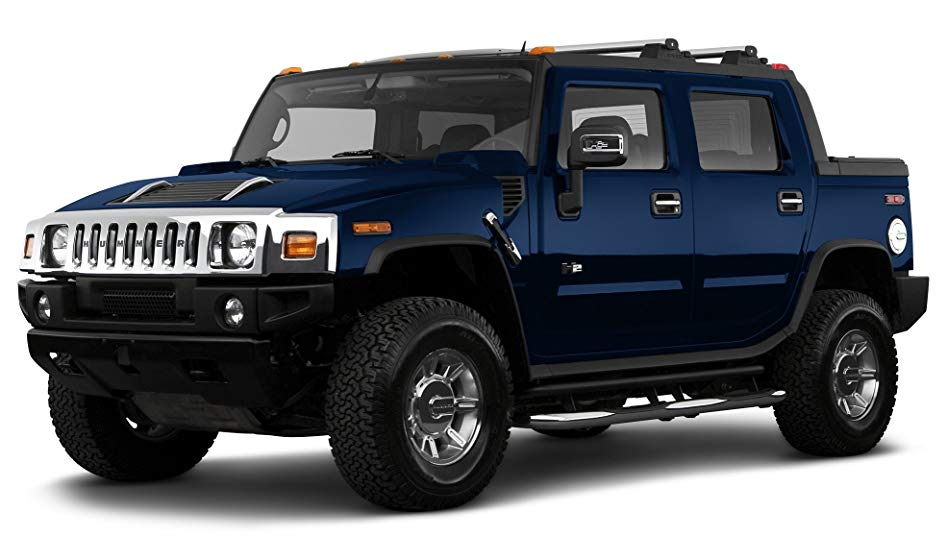
\includegraphics[width=\textwidth]{hummer.jpg}
    	\end{column}
    	\begin{column}{0.333\textwidth}
    		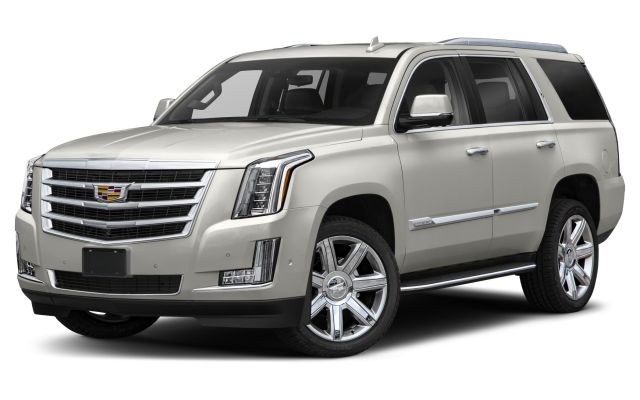
\includegraphics[width=\textwidth]{escalade.jpg}
    	\end{column}
    	\begin{column}{0.333\textwidth}
    		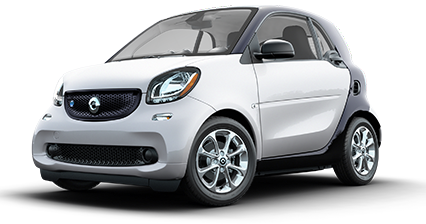
\includegraphics[width=\textwidth]{smart.png}
    	\end{column}
    \end{columns}
    \begin{columns}
    	\begin{column}{0.333\textwidth}
    		\centering Hummer H2
    	\end{column}
    	\begin{column}{0.333\textwidth}
    		\centering Cadillac Escalade
    	\end{column}
    	\begin{column}{0.333\textwidth}
    		\centering Smart Pure EV
    	\end{column}
    \end{columns}
    \vspace{3ex}
    Suppose Hummer lowers the price of the H2 to gain more market share
    \begin{itemize}
    	\item Will that attract a greater proportion of Escalade drivers or Pure EV drivers?
    	\item The logit model says that substitution to the H2 will be proportionally equal for these very different vehicles!
    \end{itemize}
\end{frame}

\begin{frame}\frametitle{Panel Data}
    If we observe panel data for a discrete choice problem, we can add a time index to our random utility model and logit choice probabilities
    $$U_{njt} = V_{njt} + \varepsilon_{njt} \quad \Rightarrow \quad P_{nit} = \frac{e^{V_{nit}}}{\sum_j e^{V_{njt}}}$$ \\
    \vspace{2ex}
    We can estimate this model just as in the cross-section
    \begin{itemize}
    	\item We can also include lagged or future variables to capture ``dynamics''
    	\item We can even include previous choices as explanatory variables to represent behavioral factors like habit formation
    \end{itemize}
    \vspace{2ex}
    The logit assumption still has to hold
    $$\varepsilon_{njt} \sim \text{i.i.d.\ type I extreme value (Gumbel) with } Var(\varepsilon_{njt}) = \frac{\pi^2}{6}$$ \\
    \begin{itemize}
    	\item But the unobserved characteristics of a decision maker that affect choice are unlikely to be independent over time
    \end{itemize}
\end{frame}

\begin{frame}\frametitle{Consumer Surplus}
    The logit model gives a closed-form expression for consumer surplus that depends on $\alpha_n$, the marginal utility of income for individual $n$
    \begin{align*}
    	CS_n &= \frac{1}{\alpha_n} \max_j (U_{nj}) \\
    	\intertext{We do not observe $U_{nj}$, but we know it in expectation}
    	E(CS_n) &= \frac{1}{\alpha_n} E\left[ \max_j (V_{nj} + \varepsilon_{nj}) \right] \\
    	\intertext{If we further assume utility is linear in income, we get}
    	E(CS_n) &= \frac{1}{\alpha_n} \ln \left( \sum_{j = 1}^J e^{V_{nj}} \right) + C
    	\intertext{So the change in consumer surplus due to changes in alternatives is}
    	\Delta E(CS_n) &= \frac{1}{\alpha_n} \left[ \ln \left( \sum_{j = 1}^{J^1} e^{V_{nj}^1} \right) - \ln \left( \sum_{j = 1}^{J^0} e^{V_{nj}^0} \right) \right]
    \end{align*}
\end{frame}

\begin{frame}\frametitle{Market-Level Data}
    The logit model can also be estimated from market-level data
    \begin{itemize}
    	\item You observe the price, market share, and characteristics of every cereal brand at the grocery store, and you want to estimate the structural parameters of consumer decision making that explain those purchases
    \end{itemize}
    \vspace{1ex}
    When aggregated over many consumers, choice probabilities become market shares
    $$S_i = \frac{e^{V_{i}}}{\sum_j e^{V_j}}$$
    If we assume representative utility is liner, $V_j = \beta' x_j$
    $$\ln(S_i) - \ln(S_j) = \beta' (x_i - x_j)$$
    Set one alternative to be your reference (usually the outside option) and estimate the linear regression for the other $J - 1$ alternatives
    $$\ln(S_i) - \ln(S_0) = \beta' (x_i - x_0) + \omega_i$$
\end{frame}

\begin{frame}\frametitle{}
    \vfill
    \centering
    \begin{beamercolorbox}[center]{title}
        \Large Multinomial Logit Model Example in R
    \end{beamercolorbox}
    \vfill
\end{frame}

\begin{frame}\frametitle{Multinomial Logit Model Example}
    We are again studying how consumers make choices about expensive and highly energy-consuming systems in their homes. We have data on 900 households in California and the type of heating system in their home. Each household has the following choice set, and we observe the following data \\
    \vspace{3ex}
    \begin{columns}
    	\begin{column}{0.5\textwidth}
		    Choice set
		    \begin{itemize}
		    	\item GC: gas central
		    	\item GR: gas room
		    	\item EC: electric central
		    	\item ER: electric room
		    	\item HP: heat pump
		    \end{itemize}
		    \vspace{8ex}
	    \end{column}
	    \begin{column}{0.5\textwidth}
		    Alternative-specific data
		    \begin{itemize}
		    	\item IC: installation cost
		    	\item OC: annual operating cost
		    \end{itemize}
		    \vspace{2ex}
		    Household demographic data
		    \begin{itemize}
		    	\item income: annual income
		    	\item agehed: age of household head
		    	\item rooms: number of rooms
                \item region: home location
		    \end{itemize}
		\end{column}
    \end{columns}
\end{frame}

\begin{frame}[fragile]\frametitle{Load Dataset}
    <<R CODE HERE>>
\end{frame}

\begin{frame}[fragile]\frametitle{Dataset}
    <<R CODE HERE>>
\end{frame}

\begin{frame}[fragile]\frametitle{Convert to a Long Dataset}
    <<R CODE HERE>>
\end{frame}

\begin{frame}[fragile]\frametitle{Long Dataset}
    <<R CODE HERE>>
\end{frame}

\begin{frame}[fragile]\frametitle{Convert Datasets to \texttt{mlogit} Format}
    <<R CODE HERE>>
\end{frame}

\begin{frame}[fragile]\frametitle{Wide Dataset in \texttt{mlogit} Format}
    <<R CODE HERE>>
\end{frame}

\begin{frame}[fragile]\frametitle{Long Dataset in \texttt{mlogit} Format}
    <<R CODE HERE>>
\end{frame}

\begin{frame}[fragile]\frametitle{Multinomial Logit Model Estimation}
    <<R CODE HERE>>
\end{frame}

\begin{frame}[fragile]\frametitle{Model Summary}
    <<R CODE HERE>>
\end{frame}

\begin{frame}[fragile]\frametitle{Elasticities}
    <<R CODE HERE>>
\end{frame}

\begin{frame}[fragile]\frametitle{Distribution of Elasticities}
    <<R CODE HERE>>
\end{frame}

\begin{frame}[fragile]\frametitle{Elasticity Distribution Plot}
    <<R CODE HERE>>
\end{frame}

\begin{frame}[fragile]\frametitle{Cross Elasticities}
    <<R CODE HERE>>
\end{frame}

\begin{frame}[fragile]\frametitle{Cost Tradeoffs}
    How do consumers trade off the installation cost and the annual operating cost?
    \begin{itemize}
        \item What reduction in installation cost offsets a \$1 increase in the annual operating cost?
    \end{itemize}
    \begin{align*}
        U_{ni} &= \alpha_i + \beta_1 IC_{ni} + \beta_2 OC_{ni} + \varepsilon_{ni} \\
        dU &= \beta_1 dIC_{ni} + \beta_2 dOC_{ni} \\
        dU = 0 \Rightarrow \frac{dIC}{dOC} &= -\frac{\beta_2}{\beta_1}
    \end{align*}
    <<R CODE HERE>>
\end{frame}

\begin{frame}\frametitle{Implied Discount Rate}
    What is the implied discount rate of consumers? Assume (for simplicity) that the operating cost accrues in perpetuity.
    \begin{align*}
        U_{ni} &= \alpha_i + \beta_1 IC_{ni} + \beta_2 OC_{ni} + \varepsilon_{ni} \\
        \intertext{Divide by $\beta_1$ to express in terms of present day dollars}
        \frac{U_{ni}}{\beta_1} &= \frac{\alpha_i}{\beta_1} + IC_{ni} + \frac{\beta_2}{\beta_1} OC_{ni} + \frac{\varepsilon_{ni}}{\beta_1} \\
        \intertext{Re-express using an infinite sum of discounted operating costs}
        \frac{U_{ni}}{\beta_1} &= \frac{\alpha_i}{\beta_1} + IC_{ni} + \frac{1}{r} OC_{ni} + \frac{\varepsilon_{ni}}{\beta_1} \\
        \intertext{The last two equations give that}
        r &= \frac{\beta_1}{\beta_2}
    \end{align*}
\end{frame}

\begin{frame}[fragile]\frametitle{Implied Discount Rate Calculation}
    <<R CODE HERE>>
\end{frame}

\begin{frame}[fragile]\frametitle{Heterogeneous Coefficients}
    <<R CODE HERE>>
\end{frame}

\begin{frame}[fragile]\frametitle{Heterogeneous Coefficients Model Summary}
    <<R CODE HERE>>
\end{frame}

\begin{frame}[fragile]\frametitle{Alternative-Specific Coefficients on Demographics}
    <<R CODE HERE>>
\end{frame}

\begin{frame}[fragile]\frametitle{Alternative-Specific Demographics Model Summary}
    \vspace{1ex}
    <<R CODE HERE>>
\end{frame}

\begin{frame}[fragile]\frametitle{Alternative-Specific Coefficients on Costs}
    <<R CODE HERE>>
\end{frame}

\begin{frame}[fragile]\frametitle{Alternative-Specific Cost Coefficients Model Summary}
    \vspace{1ex}
    <<R CODE HERE>>
\end{frame}

\begin{frame}\frametitle{}
    \vfill
    \centering
    \begin{beamercolorbox}[center]{title}
        \Large Adamowicz et al. (1994)
    \end{beamercolorbox}
    \vfill
\end{frame}

\begin{frame}\frametitle{Adamowicz et al. (1994)}
    Research question
    \begin{itemize}
    	\item Do stated preference methods and revealed preference methods yield similar results on recreational site choice?
    \end{itemize}
    \vspace{2ex}
    Empirical methods
    \begin{itemize}
    	\item Conduct both a stated preference survey and a revealed preference survey on site choice for fishing and other water-based recreation
    	\item Estimate a multinomial logit model for each model separately and a joint model including both surveys
    \end{itemize}
    \vspace{2ex}
    Results
    \begin{itemize}
    	\item Independent models appear to be different, but estimating a joint model that includes a scale parameter yields similar underlying preferences
    \end{itemize}
\end{frame}

\begin{frame}\frametitle{Stated Preference Survey}
    Method used to value non-market goods
    \begin{itemize}
    	\item Traditional application is valuing environmental amenities
    	\item Popular research method in the 1980s--2000s but less popular now
    	\item Any other areas where this could be used to elicit valuation?
    \end{itemize}
    \vspace{2ex}
    Respondents state their choice over a hypothetical set of alternatives
    \begin{itemize}
    	\item Survey methods have been refined over the years to remove bias that was present in early surveys
    	\item Do we believe hypothetical decision making reveals true preferences?
    \end{itemize}
    \vspace{2ex}
    Contrast with revealed preference methods
    \begin{itemize}
    	\item Researchers document actual choices over a set of real alternatives
    	\item May limit what parameters can be estimated
    \end{itemize}
\end{frame}

\begin{frame}\frametitle{General Comments and Questions}
    Both stated choice and revealed choice methods yield data that seem perfect for a multinomial logit model
    \begin{itemize}
    	\item But do we believe the assumptions of the logit model in this case?
    \end{itemize}
    \vspace{2ex}
    Estimation of the joint model depends importantly on the scale parameter
    \begin{itemize}
    	\item But they never say what scale parameter best fits the joint dataset
    \end{itemize}
    \vspace{2ex}
    Authors apply their results to estimate the change in consumer surplus associated with a change in river flows
    \begin{itemize}
    	\item Consumer surplus calculations require a marginal utility of income, which they do not directly estimate
    	\item Welfare effects from the joint model are much closer to the revealed preference model than to the stated preference model
    	\item What other counterfactuals or policy scenarios could we model with these results?
    \end{itemize}
\end{frame}

\begin{frame}\frametitle{Recap and Looking Ahead}
    So far
    \begin{itemize}
        \item Discrete choice framework
        \item Random utility model
        \item Logit model
    \end{itemize}
    \vspace{3ex}
    But we still do not know how to estimate the logit model! \\
    \vspace{3ex}
    Coming up
    \begin{itemize}
        \item Maximum likelihood estimation
        \item Numerical optimization
        \item Estimating the logit model
    \end{itemize}
\end{frame}

\begin{frame}\frametitle{Announcements}
    Reading for next time
    \begin{itemize}
        \item Greene textbook, Chapters 7.1--7.2.1 and 14.1--14.6
    \end{itemize}
    \vspace{3ex}
    Office hours
    \begin{itemize}
    	\item Reminder: Tuesdays at 2:00-3:00 in 218 Stockbridge
    \end{itemize}
    \vspace{3ex}
    Upcoming
    \begin{itemize}
        \item Problem Set 1 is posted, due September 24
    \end{itemize}
\end{frame}

\end{document}